\documentclass[tikz,border=3pt]{standalone}
\usepackage{xcolor}
\usetikzlibrary{arrows.meta,decorations.pathmorphing,positioning}
\definecolor{flowblue}{HTML}{2563EB}
\definecolor{reviewred}{HTML}{DC2626}
\definecolor{panelgray}{HTML}{E2E8F0}
\begin{document}
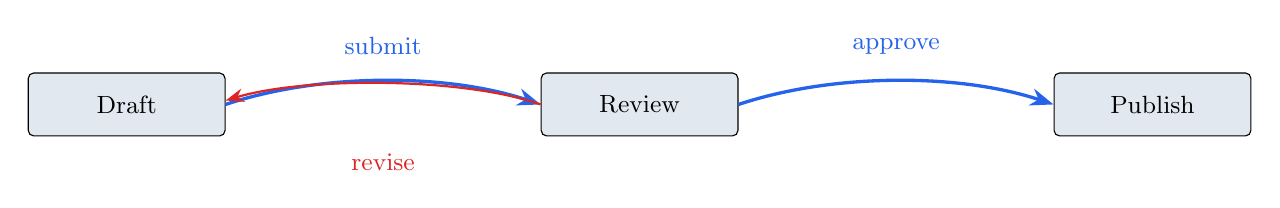
\begin{tikzpicture}[
  >=Stealth,
  stage/.style={draw,rounded corners=2pt,minimum width=2.5cm,minimum height=8mm,fill=panelgray},
  every node/.style={font=\small}
]
  \node[stage] (draft) {Draft};
  \node[stage,right=4cm of draft] (review) {Review};
  \node[stage,right=4cm of review] (ship) {Publish};
  \draw[flowblue,very thick,-Stealth,decorate,
    decoration={bent,aspect=.3,amplitude=4mm}]
    (draft) -- node[above=5mm]{submit} (review);
  \draw[flowblue,very thick,-Stealth,decorate,
    decoration={bent,aspect=.3,amplitude=4mm}]
    (review) -- node[above=5mm]{approve} (ship);
  \draw[reviewred,thick,-Stealth,decorate,
    decoration={bent,aspect=.25,amplitude=3mm,mirror,raise=.5mm}]
    (review) -- node[below=5mm]{revise} (draft);
\end{tikzpicture}
\end{document}
